\documentclass[a4paper]{article}

\usepackage[english]{babel}
\usepackage[utf8]{inputenc}
\usepackage{amsmath}
\usepackage{graphicx}
\usepackage[colorinlistoftodos]{todonotes}

\title{Project Proposal: FPGA-based Interchangeable Sensor Module for Digital Imaging}

\author{Michael Wild}

\date{\today}

\begin{document}
\maketitle

\section{Overview}

This project seeks to provide a solid base for continued work on a fully-modular digital camera system with applications in cinema, photography and computer vision.

Modern cameras (both still-motion and video) have a multitude of upgrade options: Lenses, filters and other accessories are all interchangeable, enabling creative freedom and flexibility. As one of the most important components of the system, the photographic sensor plays a vital role in the final image. It dictates not only the output resolution, but also low-light performance, colour response, frame-rate and cropping. 

In spite of its significance, only a handful of niche cinema cameras include interchangeable sensors; even then, these components are not fully modular. Upgrading the sensor in a mainstream camera requires the purchase of an entirely new system.

The aim of this project is to design a sensor-agnostic interface which can be used to connect any sensor to any processing board, thus providing a truly modular and upgradeable camera system.

\section{Goals}

\begin{itemize}
\item Functional prototype 
\item Sensor-agnostic interface and image acquisition pipeline
\item Support fixed image resolution and frame rate (1080p/24)
\item Ability to acquire live video from sensor
\item Storage through either external HDMI recorder or flash
\end{itemize}

\section{Required Facilities}

EDA software and SMD soldering equipment will be required for the design and manufacture of a custom image sensor PCB as well as high-performance test equipment for analysing data buses. Additionally, extensive use of 3D printing will be required in the later stages of the project to produce a protective housing for the sensor.

\section{Knowledge Areas}

\begin{itemize}
\item Image Processing
\item FPGA Design
\item Embedded Linux
\item PCB Design
\item High-Speed Interfaces
\end{itemize}

\section{Implementation}

A preliminary system is presented in Figure \ref{fig:system} which will be able to capture image data from a sensor and store it in flash using a Xilinx Zynq SoC in combination with a custom-designed interchangeable sensor board based on the CMV12000 sensor from CMOSIS.

\begin{figure}
\centering
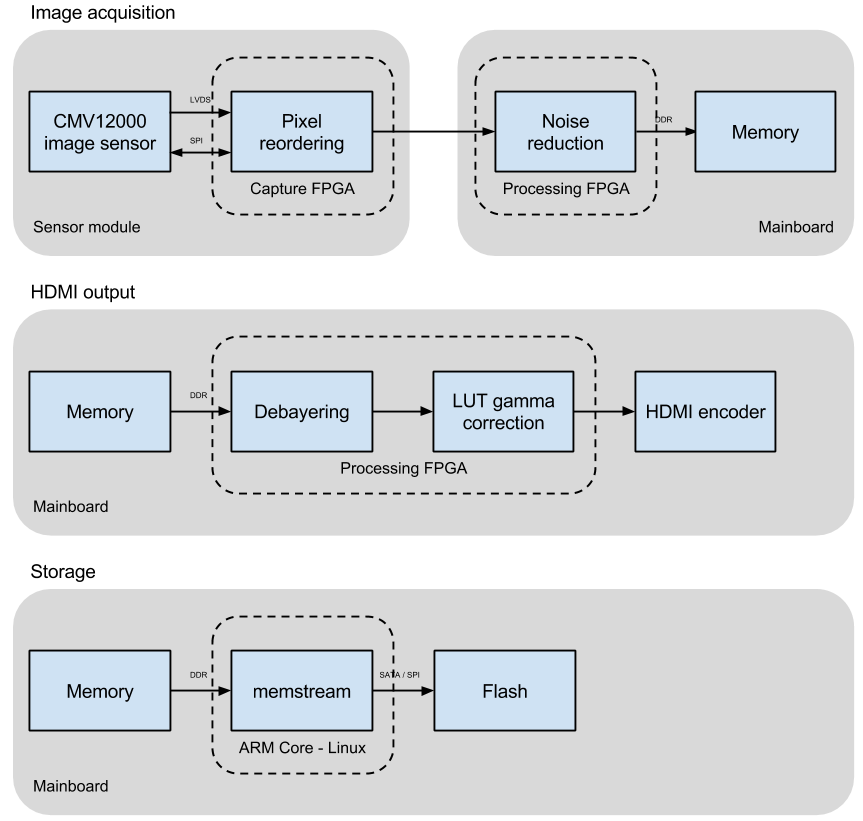
\includegraphics[width=1\textwidth]{system.png}
\caption{\label{fig:system}High-level overview of system to capture and store image data.}
\end{figure}

\end{document}